% BACKGROUND sec:background %%%%%%%%%%%%%%%%%%%%%%%%%%%%%%%%%%%%%%%%%%%%%%%%%%%%%%%%%%%%%%%%%%
In this section, we provide information on the necessary tensor properties and operations, and then introduce tensor decompositions and associated randomized methods.
%
\subsection{Tensors}
A tensor is an element in a tensor product of vector spaces. In data analysis, 
it suffices to think about a tensor as a multidimensional array.
We represent a tensor as a Euler script capital letter, e.g., 
$\T{X}\in \R^{n_1 \times \cdots \times n_d}$. 

The number of \emph{modes} (or dimensions) of a tensor is referred to as its \emph{order}, 
denoted by $d$. The values $n_k$ denote the dimensions of a tensor, and we let $n=\sqrt[d]{\prod_k n_k}$, 
so that $n^d = \prod_k n_k$. Thus, the term $n^d$ to more intuitively expresses the number of elements 
 in a tensor as exponential in its order. We also let $n_k^\oslash = n^d / n_k$ represent the product of all 
 dimensions \emph{except} $n_k$.

Let $\mathcal{I} = \{ \V{i} = (i_1,\dots,i_d) \}$ be the set of indices of a tensor. 
We can thus express an individual element of a tensor $\T{X}$ for any multiindex $\V{i}$ as $x_{\V{i}}$. 

The \emph{mode-$k$ fibers} of a tensor are higher-order analogues
of matrix columns and rows.
The mode-$k$ \emph{unfolding} or \emph{matricization} of a tensor 
aligns the mode-$k$ fibers as the columns of an $n_k \times n_k^\oslash$ matrix. 
Assuming 1-indexing, tensor entry $x_{\mathbf{i}}$ then maps to
entry $(i_k, j)$ of $\M{X}_{(k)}$ via the relation: 
\begin{equation}
  \label{eqn:unfoldmapping}
  j = 1+\sum_{\substack{\ell=1\\\ell\neq k}}^d (i_\ell -1)m_\ell, \qquad \text{where} \qquad m_\ell = \prod_{\substack{q=1\\q\neq \ell}}^{\ell-1} n_q.
\end{equation}
The \emph{norm} of a tensor is the square root of the sum of its squared entries, 
e.g., $\|\T{X}\| = \|\M{X}_{(k)}\|_F$ for any $k$. Given a decomposed representation $\T{M}$ of a tensor,
the normalized residual error can be written as:
\begin{equation}
\|\T{X}-\T{M}\|/{\|\T{X}\|}
\end{equation}
Given matrices $\M{A} \in \mathbb{R}^{n_1 \times n_2}$ and $\M{B} \in \mathbb{R}^{m_1
  \times m_2}$, their \emph{Kronecker product} is 
\begin{displaymath}
  \M{A} \otimes \M{B} =
  \begin{bmatrix}
    a_{11} \M{B} & a_{12} \M{B} & \cdots & a_{1n_2} \M{B} \\
    \vdots & \vdots & \ddots & \vdots \\
    a_{n_1 1} \M{B} & a_{n_1 2} \M{B} & \cdots & a_{n_1 n_2} \M{B} \\
  \end{bmatrix}
  \in \R^{n_1 m_1 \times n_2 m_2}.
\end{displaymath}
%
Assuming $n_2 = m_2$, their \emph{Khatri-Rao product}, also known as the
\emph{matching columnwise Kronecker product}, is
\begin{displaymath}
  \M{A} \odot \M{B} = 
  \begin{bmatrix}
    \V{a}_1 \otimes \V{b}_1 & \V{a}_2 \otimes \V{b}_2
    & \cdots &  \V{a}_J \otimes \V{b}_J \in \mathbb{R}^{n_1 m_1 \times n_2}.   
  \end{bmatrix}
\end{displaymath}
Assuming $n_1=m_1$ and $n_2=m_2$, their \emph{Hadamard product} is
$\M{A}\circledast\M{B} \in \mathbb{R}^{n_1 \times n_2}$, the elementwise product of the matrices.
Three useful identities involving the products just defined are:
\begin{align}
(\M{A} \odot \M{B})^\trans(\M{A} \odot \M{B}) &= \M{A}^\trans\M{A} \circledast \M{B}^\trans\M{B}, \label{eq:KRGram} \\ 
\M{A}\M{B} \otimes \M{C}\M{D} &= (\M{A} \otimes \M{C})(\M{B} \otimes \M{D}) \label{eqn:krondist},\quad\text{and} \\
\M{A}\M{B} \odot \M{C}\M{D} &= (\M{A} \otimes \M{C})(\M{B} \odot \M{D}). \label{eqn:krdist}
\end{align}

%
The \emph{mode-$k$ tensor-times-matrix product} (TTM) is a contraction
between a matrix and a tensor in its $k$th mode.
\begin{equation}
\label{eqn:ttm}
\T{Y} = \T{X} \times_k \M{A} \quad \Leftrightarrow \quad \M{Y}_{(k)} = \M{A}\M{X}_{(k)}.
\end{equation}
We can also write this element-wise as
\begin{equation}
  \label{eqn:contractionelem}
  y_{i_1i_2\cdots i_{k-1}j i_{k+1}\cdots i_d} = \sum_{i_k}x_{i_1\cdots i_d}u_{j i_k}
\end{equation}
We will use bracket notation to denote multiple products, e.g. 
$\T{X} \times \{\Mn{U}{k}\}$ refers to $\T{X}$ multiplied by $\Mn{U}{k}$ 
for every $k=1,\dots,d$. The result is invariant to which order the TTMs are performed in, 
providing the modes are unique. If a tensor can be written as a series of 
mode-$k$ products, its mode-$k$ matricization has a particular structure~\cite{Kolda:2009}:
\begin{align}
  \begin{split}
    \label{eqn:ttensor}\T{Y} & ={}  \T{X} \times \{\Mn{U}{k}\} \quad \Leftrightarrow \\
    \M{Y}_{(k)} & ={}  \Mn{U}{k} \M{X}_{(k)} 
    (\Mn{U}{d} \otimes \cdots \otimes \Mn{U}{k+1} \otimes \Mn{U}{k-1} \otimes \cdots \otimes \Mn{U}{1})^\trans.
  \end{split}
\end{align}
%
\begin{table}[ht]
  \centering%\footnotesize
  \label{tab:notation}
  \begin{tabular}{cl}
    \toprule
    Notation & Definition \\
    \midrule
    $\M{X}_{(k)}$ & mode-$k$ unfolding of $\T{X}$ \\
    $\T{X}\times_k \M{U}_k$ & Tensor-Times Matrix Multiplication (TTM) \\
    $\M{A}\otimes\M{B}$ & Kronecker Product \\
    $\M{A}\odot\M{B}$ & Khatri-Rao Product \\
    $\M{A}\circledast \M{B}$ & Hadamard Product \\
    \midrule
    $d$ & Number of modes (order) of a tensor \\
    $n_k$ & Size of mode $k$ of tensor $\T{X}$ \\
    $r_k$ & Rank (core size) of mode $k$\footnote{For the CP decomposition there is only one rank $r$} \\
    $p_k$ & Number of processors along mode $k$ \\
    $s_k$ & Sketch size of mode $k$ \\
    $n,r,p,s$ & $\sqrt[d]{\prod n_k}, \sqrt[d]{\prod r_k}, \sqrt[p]{\prod p_k}, \sqrt[d]{\prod s_k}$ \\
    $n_k^\oslash,r_k^\oslash,p_k^\oslash,s_k^\oslash$ & $n^d/n_k,r^d/r_k,p^d/p_k,s^d/s_k$ \\
    % \midrule
    % $\Mn{U}{k}\in\mathbb{R}^{n_k\times r_k}$ & Tucker factor matrix for mode $k$ \\
    % $\M{\Omega}_k\in\mathbb{R}^{n_k \times s_k}$ & Random sketch matrix for mode $k$ \\
    % $\T{G}\in\mathbb{R}^{r_1\times\cdots\times r_d}$ & Tucker core \\
    % $\T{M} = \{\T{G},\{\M{U}_k\} \}$ & Tucker approximation of $\T{X}$ \\
    % $\bar{\T{X}}$ & Local subtensor of $\T{X}$ \\
    \bottomrule
  \end{tabular}
  \caption{Basic tensor notation used in this proposal.}
\end{table}
%
\subsection{CP Decomposition}
The CP tensor decomposition aims to approximate an order-$d$ tensor as
a sum of $r$ rank-one
tensors~\cite{hitchcock-sum-1927, CANDECOMP, PARAFAC, Kolda:2009}:  
\begin{equation}
\label{eqn:cpform}
\T{X} \approx \T{\tilde{X}} = \sum_{k=1}^d \V{a}_k^{(1)} \circ \V{a}_k^{(2)} \circ \cdots \circ \V{a}_k^{(d)},
\end{equation}
where \emph{factor vector} $\V{a}_r^{(k)}$ has length $n_k$. 
Each rank-one tensor is called a \emph{component}.
The collection of all factor vectors for a given mode is called a 
\emph{factor matrix}:
\begin{displaymath}
  \Mn{A}{k} =
  \begin{bmatrix}
    \MnC{A}{k}{1} &
    \MnC{A}{k}{2} &
    \cdots &
    \MnC{A}{k}{r}
  \end{bmatrix}
  \in\R^{n_k \times r}.
\end{displaymath}
The mode-$k$ matricization of $\T{\tilde{X}}$ can be written in terms
the factor matrices as
\begin{equation}\label{eq:Zn}
  \M{\tilde{X}}_{(k)} = \M{A}^{(k)}\M{Z}^{(k)\trans}
  \qtext{where}
  \M{Z}^{(k)}=\M{A}^{(d)}\odot \cdots  \M{A}^{(k+1)}\odot
  \M{A}^{(k-1)} \odot \cdots \odot \M{A}^{(1)}.   
\end{equation}
We may alternatively represent \cref{eqn:cpform} by normalizing all
the factor vectors to unit length and expressing the product of the
normalization factors as a scalar weight $\lambda_r$ for each
component: 
\begin{equation}\label{eq:cpformlambda}
  \T{\tilde{X}} = \sum_{k=1}^d \lambda_k \; \V{a}_k^{(1)} \circ
  \V{a}_k^{(2)} \circ \cdots \circ \V{a}_k^{(d)}.
\end{equation}

\subsubsection{CP-ALS}

The standard method for fitting the CP model is alternating least
squares (CP-ALS) \cite{PARAFAC,Kolda:2009}. The method alternates
among the modes, fixing every factor matrix but $\Mn{A}{k}$ and
solving for it. From \cref{eq:Zn}, 
we see that we can find $\Mn{A}{k}$ by solving the linear least squares
problem given by
\begin{equation}
\label{eq:lls}
\argmin_{\M{A}^{(k)}} \|\M{X}_{(k)} - \M{A}^{(k)}\M{Z}^{(k)\trans}\|_F.
\end{equation}
In CP-ALS, we work with the normal equations for \cref{eq:lls}:
\begin{displaymath}
\M{X}_{(k)}\M{Z}^{(k)} = \M{A}^{(k)}(\M{Z}^{(k)\trans}\M{Z}^{(k)}),
\end{displaymath}
and solve for $\M{A}^{(k)}$ for given $\M{X}_{(k)}$ and $\M{Z}^{(k)}$.
By identity \cref{eq:KRGram}, we have 
\begin{displaymath}
\M{Z}^{(k)\trans}\M{Z}^{(k)} = \M{A}^{(d)\trans}\M{A}^{(d)} \circledast \dots \circledast \M{A}^{(k+1)\trans}\M{A}^{(k+1)} \circledast \M{A}^{(k-1)\trans}\M{A}^{(k-1)} \circledast \cdots \circledast \M{A}^{(1)\trans}\M{A}^{(1)}.
\end{displaymath}

The CP-ALS algorithm~\cite{Kolda:2009} is presented
in~\cref{alg:cpals}. Note the step where vector $\bm{\lambda}$ stores
normalization values of each column so that the final approximation is
as in \cref{eq:cpformlambda}; this normalization helps alleviate
issues due to scaling ambiguity.

The initialization of the factor matrices
can impact the performance of the algorithm.
There are many possible ways to do the the initialization.
One way is to
initialize is to set $\Mn{A}{k}$ to be the leading $r$ left singular
vectors of the mode-$k$ unfolding, $\M{X}_{(k)}$, and we call this
HOSVD initialization, as it corresponds to the factor matrices
in the rank-$(r{\times} {\cdots} {\times} r)$ HOSVD (see~\cref{sec:hosvd}). 
A less expensive but less effective initialization is to
choose random factor matrices.

\begin{algorithm}
  \caption{CP-ALS}
  \label{alg:cpals}
  \begin{algorithmic}[1]\footnotesize
    \Function{$[\bm{\lambda},\set{\M{A}^{(n)}}]=$ CP-ALS}{$\T{X},R$}\Comment{$\T{X}\in\mathbb{R}^{I_1\times \cdots \times I_N}$}
    \State \label{line:cpals:init} Initialize factor matrices $\M{A}^{(2)}, \dots, \M{A}^{(N)}$
    \Repeat
    \For{$n=1,\dots, N$}
      \State $\M{V} \gets \M{A}^{(N)\trans}\M{A}^{(N)} \circledast \dots \circledast \M{A}^{(n+1)\trans}\M{A}^{(n+1)} \circledast \M{A}^{(n-1)\trans}\M{A}^{(n-1)} \circledast \cdots \circledast \M{A}^{(1)\trans}\M{A}^{(1)}$\label{line:cpals:Gram}
      \State \label{line:cpals:KR} $\M{Z}^{(n)} \gets \M{A}^{(N)}\odot \cdots  \odot \M{A}^{(n+1)}\odot \M{A}^{(n-1)} \odot \cdots \odot \M{A}^{(1)}$
      \State \label{line:cpals:MTTKRP} $\M{W} \gets \M{X}_{(n)}\M{Z}^{(n)}$
      \State \label{line:cpals:solve} Solve $\M{A}^{(n)}\M{V} = \M{W}$ for $\M{A}^{(n)}$        
      \State Normalize columns of $\M{A}^{(n)}$ and update $\bm{\lambda}$
    \EndFor
    \Until termination criteria met
    \State \textbf{return} $\bm{\lambda}$, factor matrices $\set{\M{A}^{(n)}}$
    \EndFunction
  \end{algorithmic}
\end{algorithm}


\subsection{The Tucker Decomposition} \label{sec:hosvd} 
\begin{figure}[htbp]
  \centering
\begin{tikzpicture}[scale=0.5,namenode/.style={scale=.75}]
	\def\ix{3} %
	\def\iy{3} %
	\def\iz{2.5} %
	\def\corescale{1.75}
	\def\rx{\ix/\corescale}
	\def\ry{\iy/\corescale}
	\def\rz{\iz/\corescale}
	\coordinate (XFrontLowerLeft) at (0,0);
	\draw (XFrontLowerLeft) rectangle ++ (\ix,\iy); %
	\begin{scope}[shift={(XFrontLowerLeft)},canvas is zx plane at y=\iy,rotate=90]
	  \draw (0,0) rectangle ++ (\ix,\iz); %
	\end{scope}
	\begin{scope}[shift={(XFrontLowerLeft)},canvas is zy plane at x=\ix,rotate=90]
	  \draw (0,0) rectangle ++ (\iy,\iz); %
	\end{scope}
	\node[namenode] at ($(XFrontLowerLeft) + (0.5*\ix, 0.5*\iy)$)  {$\T{X}$};
	\coordinate (ApproxCtr) at ($(XFrontLowerLeft) + (\ix+0.4*\iz,0.75*\iy) + (0.75,0)$);

	\node[namenode] at (ApproxCtr) {$\approx$};
	\coordinate (U1LowerLeft) at ($(ApproxCtr) - (0,0.75*\iy) + (0.75,0)$);
	\draw (U1LowerLeft) rectangle ++ (\ry,\iy);

	\node[namenode] at ($(U1LowerLeft)+(0.5*\ry, 0.5*\iy)$)  {$\Mn{U}{1}$};
	\coordinate (GFrontLowerLeft) at ($(U1LowerLeft) + (\ry+0.5,1)$);
	\draw (GFrontLowerLeft) rectangle ++ (\rx,\ry);
	\begin{scope}[shift={(GFrontLowerLeft)},canvas is zx plane at y=\ry,rotate=90]
	  \draw (0,0) rectangle ++ (\rx,\rz);
	\end{scope}
	\begin{scope}[shift={(GFrontLowerLeft)},canvas is zy plane at x=\rx,rotate=90]
	  \draw (0,0) rectangle ++ (\ry,\rz);
	\end{scope}
	\node[namenode] at ($(GFrontLowerLeft)+(0.5*\rx,.5*\ry)$)  {$\T{G}$};
	\coordinate (U2LowerLeft) at ($(GFrontLowerLeft) + (\rx+\rz*0.4+0.5,0.5)$);
	\draw (U2LowerLeft) rectangle ++ (\ix,\rx); %

	\node[namenode] at ($(U2LowerLeft)+(0.5*\ix,0.5*\rx)$)  {$\Mn{U}{2}$};
	\coordinate (U3LowerLeft) at ($(GFrontLowerLeft) + (0.5,\ry+.8)$);
	\begin{scope}[shift={(U3LowerLeft)},canvas is zx plane at y=0,rotate=90]
	  \draw (0,0) rectangle ++ (\rz,\iz); %
	\end{scope}
	\node[namenode] at ($(U3LowerLeft)+(1.2,0.5)$) {$\Mn{U}{3}$};
\end{tikzpicture}
  \caption{Tucker decomposition of 3rd-order tensor ($d=3$).}
  \label{fig:thirdordertucker}
\end{figure}
%%% Local Variables:
%%% mode: latex
%%% TeX-master: t
%%% End:
 %%%%%% Tucker Figure %%%%%%
The Tucker decomposition~\cite{Tu66} approximates a tensor with a core tensor contracted with 
matrices in each mode:
\begin{displaymath}
  \T{X} \approx \T{M} = \T{G} \times_1 \Mn{U}{1} \times_2 \Mn{U}{2} \cdots \times_d \Mn{U}{d} = \T{G} \times \{\Mn{U}{k}\},
\end{displaymath}
where
$\T{G}$ is a dense core of size $r_1 \times r_2 \times \cdots \times r_d$, and the factor matrices 
$\Mn{U}{k}$ have size $n_k \times r_k$ for $k=1, \dots, d$.

The \hosvd~\cite{Lathauwer00amultilinear} is a method for computing the Tucker decomposition that computes a series 
of SVDs of
unfolded tensors to compute the orthogonal factor matrices $\Mn{U}{k}$ whose 
columns approximately span the columns of the unfolded tensor $\M{X}_{(k)}$ for each mode $k$. We will refer to this computation as the Mode-wise Truncated Fiber Space Basis Computation (\MTFSBC).
Following this operation, the resulting factor matrices are applied to the input tensor to compress the original data into the core $\T{G}$: $\T{G} \gets \T{X} \times \{ \Mn{U}{k} \}$. 

Just as we would compress a matrix by truncating its SVD, we can truncate the factors 
$\Mn{U}{k}$ so that $\T{G}$ is a smaller core ($r_k < n_k$), a method we refer to as the 
\emph{truncated} \hosvd (\thosvd), presented in~\cref{alg:sthosvd}.
This is particularly effective for compression; as with $n$, we let $r=\sqrt[d]{\prod r_k}$, and so 
the core is exponentially smaller than $\T{X}$, a factor of $(\frac{n}{r})^d$. 
The total compression ratio includes the factor matrices:
\begin{equation}
\label{eqn:compression}
n^d / \left(r^d + \sum_{k=1}^d n_k r_k\right).
\end{equation}

The HOSVD can be
implemented by forming the $n_k \times n_k$ Gram matrix $\M{S}_k = \M{X}_{(k)}\M{X}_{(k)}^\trans$ 
and computing its eigendecomposition. The eigenvectors of $\M{S}_k$ correspond to the left
singular vectors of $\M{X}_{(k)}$, and $\lambda_j(\M{S}_k) = \sigma_j(\M{X}_{(k)})^2$. 
This Gram computation is utilized by TuckerMPI, which performs a distributed Gram matrix 
computation followed by a local eigendecomposition~\cite{AuBaKo16}.
We use the Gram variant because we 
assume that dimensions are reasonably-sized, e.g., $n_k \leq 10^4$ for all $k$.

\begin{algorithm}[htb]
  \caption{\thosvd\Comment{Gram Variant}}
  \begin{algorithmic}[1]
    \Procedure{\thosvd}{$\T{X}$, $(r_1,\dots,r_d)$}
    \For{$k=1,\dots,d$}
    % \State $[\M{U},\M{\Sigma}] \gets \text{SVD}(\M{X}_{(k)})$
    \State $\M{S}_k \gets \M{X}_{(k)}\M{X}_{(k)}^\trans $ \Comment{Gram}
    \State $[\M{U},\M{\lambda}] \gets \text{eig}(\M{S}_k)$ \Comment{Eigensolve}
    % \State $r_k \gets $ min $j$ s.t. $\sum_{r>j} \lambda_r \leq \epsilon^2\|\T{X}\|^2/d$
    \State \label{line:sthosvd:svd} $\Mn{U}{k} \gets \text{ leading $r_k$ eigenvectors in $\M{U}$}$
    \EndFor
    \State \label{line:sthosvd:trunc} $\T{G} \gets \{ \T{X} \times \Mn{U}{k}^\trans\}$ \Comment{TTM (Core Formation)}
    \State $\T{M} \gets \{ \T{G}, \set{\Mn{U}{k}} \}$ \label{line:sthosvd:ttm}
    \State \Return $\T{M}$
    \EndProcedure
  \end{algorithmic}
  \label{alg:sthosvd}
\end{algorithm}
%
A new variant of the \thosvd is the \emph{sequentially} truncated \hosvd (\sthosvd)~\cite{sthosvd}, 
which is implemented in TuckerMPI~\cite{AuBaKo16}. Whereas the \thosvd forms the core 
after performing the \MTFSBC for all modes (in~\cref{line:sthosvd:ttm}), 
the \sthosvd performs a \MTFSBC for a single mode followed by a core-compression step in that mode,
such that the $k$th TTM occurs within the $k$th iteration of the for loop. 
The working size of the tensor thus reduces by a 
factor of $n_k / r_k$ at each iteration, with an equivalent reduction in the cost of subsequent SVD steps.
%
\subsection{Tensor Train Decomposition}
The Tensor Train decomposition (TT) factors an order-$d$ tensor into a set of $d$ tensors. The $k$th tensor is denoted $G^{(k)}$, where $G^{(1)}$ and $G^{(d)}$ are of order 2, and all other tensors are of order 3. 

The input tensor can then be reconstructed via the relation:
\begin{equation}
\T{X} \approx \M{G}^{(1)} \times_{2}^1 \T{G}^{(2)} \times_{3}^1 \T{G}^{(3)} \times_3^1 \dots
\times_3^1 \T{G}^{(d-1)}\times_3^1 \M{G}^{(d)} 
\end{equation}
where $\T{X} \times_a^b \T{Y}$ can be computed as $\M{X}_b \M{Y}_a$, or more generally as 
\begin{align*}
\T{X}(i_1,\dots,i_d) & \approx  
\sum_{{k_1}=1}^{r_1} \sum_{{k_2}=1}^{r_2}\cdots\sum_{{k_{d-1}}=1}^{r_{d-1}} \T{G}^{(1)}(i_1,k_1)\T{G}^{(2)}(k_1,i_2,k_2) & \\ & \cdots\T{G}^{(d-1)}(k_{d-2},i_{d-1},k_{d-1})\T{G}^{(d)}(k_{d-1},i_d)
\end{align*}
where $\M{G}^{(1)}\in \R^{r_1\times n_1}$, $\T{G}^{(k)} \in \R^{r_{k-1}\times n_k \times r_k}$ for $1< k< d$ and $\M{G}^{(d)}\in \R^{R_{d-1}\times n_d}$. The relationship between tensors can be better understood in terms of a tensor network diagram. In this visualization, each node represents a tensor, and each line represents a mode, with the associated mode size. Lines that connect tensors represent the common mode that can be contracted to reconstruct the input tensor:
\begin{figure}[htbp]
    \center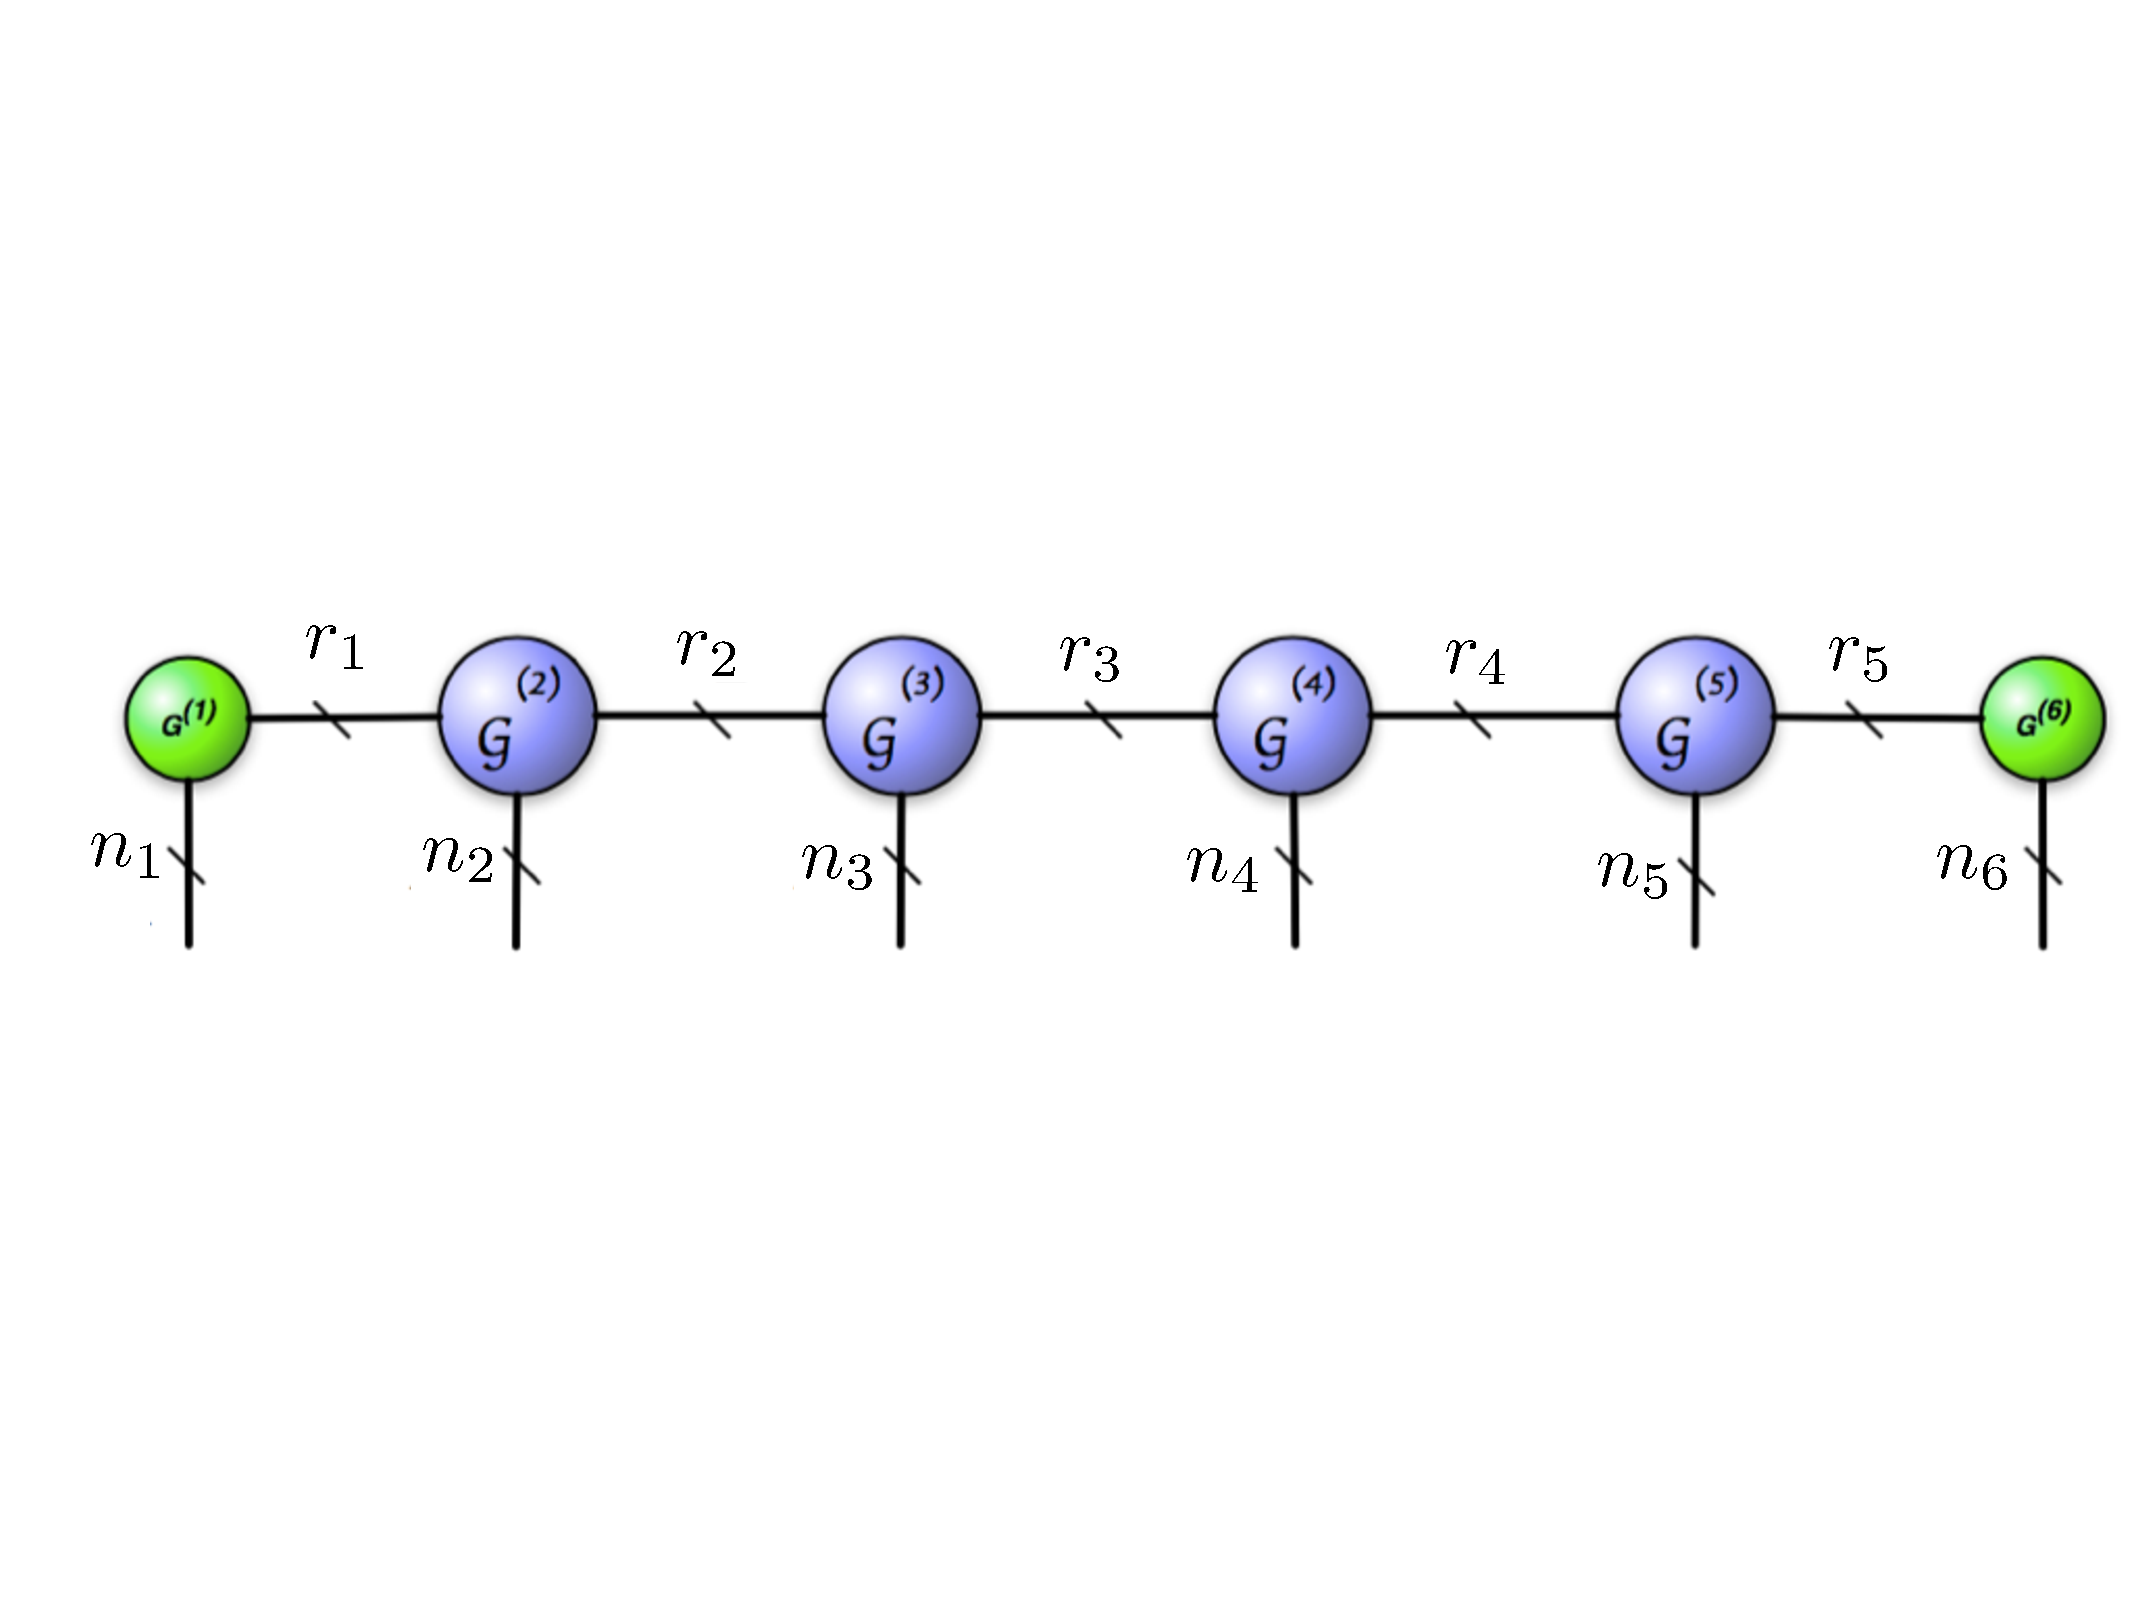
\includegraphics[width=0.80\linewidth]{thpropfigs/tensortrain}
    \caption{Tensor Train Decomposition}
\end{figure}
Computing this representation involves a straightforward recursive application of matricization and the skinny SVD.
\subsection{Randomized Least Squares}
\subsection{Randomized SVD}
%
%
%
%
%
%
%
\section{Literature Survey}
A broad survey of tensor decompositions is provided by Kolda and Bader~\cite{Kolda:2009}. Additional surveys outline specific tensor techniques in machine learning~\cite{nikossurvey}, quantum chemistry~\cite{quantumsurvey}, latent variable models~\cite{Anandk}, and neuroscience~\cite{eegsurvey}. In this proposal we will focus on scalable implementations of three of the most popular tensor decompositions: the \textsc{Candecomp/Parafac} (CP) decomposition~\cite{hitchcock-sum-1927, CANDECOMP, PARAFAC}, the Tucker decomposition~\cite{Tu66}, and the Tensor Train decomposition~\cite{tensortrain}. 

\paragraph{Sketching}
Sketching is a technique for solving linear algebra problems by constructing a smaller problem whose solution is a reasonable approximation to the original problem with high probability~\cite{sketching}. For instance, a large matrix may be sketched by applying random sampling or random projections to form a smaller sketch matrix. While this approach is suitable for a wide variety of problems, we will focus on two essential building blocks: randomized least squares~\cite{rokhlintygert,DrMaMuSa11,blendenpik}, and the randomized SVD~\cite{halko}. 


